\section{Pilotforsøg} \label{sec:pilotforsoeg}
I dette bilag beskrives pilotforsøgets fremgangsmåde samt, hvilke resultater, der opsamles. 

\subsection{Formål}
Dette pilotforsøg har til formål at kunne præcisere samt optimere kravspecifikationerne i de enkelte blokke, hvorved uklare parametre forventes besvaret ud fra pilotforsøgets resultater. Disse parametre omfatter identificering af støjsignaler samt EMG-signalets frekvensområde, da der ses variation i liiteraturen. Parametrene vil forsøges besvaret ud fra målinger ved udførelse af en squat-øvelse.
Hertil anvendes elektroder og to accelerometre som sensorer. På baggrund af dette opstilles følgende formål:  

\subsubsection{EMG-måling}
\begin{enumerate}
\item Opsamling af signal fra rectus femoris % og biceps femoris
	\begin{itemize}
	\item Identificering af frekvensområde
	\item Identificering af støjsignaler 
	\end{itemize}
%\item Identificering af gain til mikroprocesserens operationsspænding \fxnote{Finde operationsspænding og angiv den her}
\end{enumerate}

\subsubsection{Accelerometer-måling}
\begin{enumerate}
\item Identificering af støjsignaler 
\item Identificering af knæleddets vinkel
\end{enumerate}

\subsection{Materialer} 
\begin{itemize}
\item EMG-forstærker, Muscle Sensor V3
\item Elektroder
\item Desinfektionsservietter
\item Skraber
\item To accelerometre ADXL335Z
\item Tape
\item Tusch
\item Breadboards
\item Linial 
\item Vinkelmåler
\item Computer med Scopelogger og MATLAB
\item Ni USB-6009
\item USB-isolater USI-01
\end{itemize}

\subsection{Forsøgsopstilling}
%Til forsøget benyttes to EMG-forstærkere. Dette giver to sæt elektroder til differensmåling af henholdsvis rectus femoris og biceps femoris. Hvert sæt elektroder består af én positiv-, negativ- samt én referenceelektrode. 
%For at identificere elektrodeplacering på musklerne tages der udgangspunkt i Seniam's anvisning for elektrodeplacering \citep{seniam2016}. 
%Elektoderne placeres midt for linjen mellem ischial tuberosity og den laterale epifyse af tibia ved måling over biceps femoris. Ved måling af rectus femoris placeres elektroderne midt for linjen mellem anterior spina iliaca superior og den superior del af patella \citep{seniam2016}. Placeringen af elektroderne illustreres af \autoref{fig:laarmuskler}. 

Til forsøget benyttes en EMG-forstærker, der måler en differensmåling over rectus femoris. Hertil anvendes én positiv-, negativ- samt én referenceelektrode. Forinden påsættelse af elektroder, prepereres huden for således at fjerne hår samt døde hudceller.
For at identificere elektrodeplacering på musklen tages der udgangspunkt i SENIAM's anvisning for elektrodeplacering \citep{seniam2016}. 
Elektoderne placeres midt for linjen mellem anterior spina iliaca superior og den superior del af patella \citep{seniam2016}. Placeringen af elektroderne illustreres af \autoref{fig:laarmuskler}.

\begin{figure}[H]
\centering
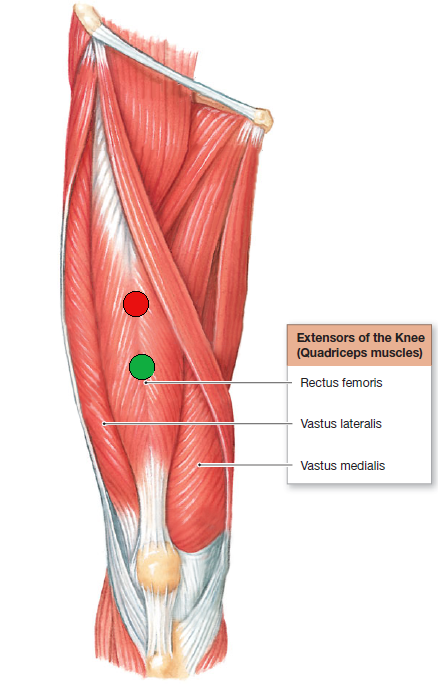
\includegraphics[width=0.3\textwidth]{figures/laarmuskel.png}
\caption{Låret set anteriot. Placering af positiv (rød) samt negativ (grøn) elektrode ses på rectus femoris \citep{martini2012}.}
\label{fig:laarmuskler}
\end{figure}

Referenceelektroden placeres, ligeledes efter SENIAM's anvisninger, omkring anklen \citep{seniam2016}. Placeringen af reference elektroden ses af \autoref{fig:reference}.

\begin{figure}[H]
\centering
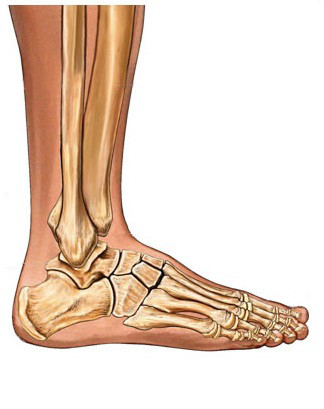
\includegraphics[width=0.3\textwidth]{figures/reference}
\caption{Placering af referenceelektrode omkring anklen \citep{ankle2016}.}
\label{fig:reference}
\end{figure}

Til forsøget benyttes endvidere to accelerometre, som måler i X-, Y- samt Z-aksen. Disse benyttes for at kunne identificere vinklen af knæet under øvelsen. For så vidt muligt at kunne stabilisere accelerometrene under udførelsen af forsøget, placeres disse på breadboards. 
Som det fremgår af \autoref{fig:accelerometervinkel} placeres det ene accelerometer midt på den laterale side af låret, parallelt med femur. Det andet accelerometer placeres midt på den laterale side af underbenet, parallelt med tibia. Disse breadboards påsættes benet ved brug af tape. Knæets vinkel i oprejst position måler 180$^{\circ}$, hvilket svarer til en 0 g-påvirkning. Vinklen af knæet ændres i takt med udførelse af en squat-øvelse, hvorved g-påvirkningen bevæger sig mod 1. Den samlede vinkel af knæet bestemmes ud fra de to accelerometres parametre. Udregningen for dette kan ses i \autoref{sec:test_acc}.

\begin{figure}[H]
\centering
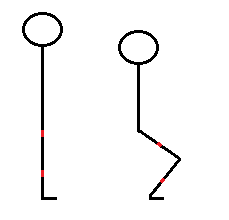
\includegraphics[width=0.4\textwidth]{figures/accelerometervinkel.png}
\caption{Placering af accelerometrene på låret samt underbenet. Disse placeringer er markeret med rød. Personen til venstre står i oprejst position, hvilket svarer til at knæets vinkel er 180 $^{\circ}$. Personen til højre sidder i en squat-øvelse, hvilket svarer til knæets vinkel som maksimalt er 90 $^{\citc}$.}
\label{fig:accelerometervinkel}
\end{figure}

Til identificering af støj fra EMG-forstærkeren fortages der baselinemålinger, som senere analyseres via en frekvensanalyse. Det samme gør sig gældende for identificeringen af EMG-signalets frekvensområde. Dette vil foregå under udførelsen af en squat-øvelse.
En squat-øvelse defineres, således den kan gengives på tværs af forsøgspersonerne.\vspace{3mm}
\begin{enumerate}
\item Forsøgspersonen står i oprejst position. Fødderne placeres med en afstand svarende til ens skulderbredde, hvortil tåspidserne peges let til siderne
\item Armene placeres over kors, som vist på \autoref{fig:squat}
\item Hofte og knæ bøjes således kroppen sænkes kontrolleret. Dette fortsættes indtil en vinkel på maksimalt 90$^{\circ}$ af knæet er opnået.
	\begin{itemize}
	\item Ryggen holdes ret under squat-øvelsen 
	\item Knæene må ikke gå ud over tåspidserne 
	\end{itemize}
\item Kroppen returneres til udgangspunksposition
\end{enumerate} \vspace{3mm}
En illustration af squat-øvelsen ses af \autoref{fig:squat}.

En nedadgående squat-øvelse defineres som punkt $1-2$ i overstående, hertil forbliver forsøgspersonen i en siddende squat indtil den givene måling er gennemført.

For at præcisere øvelsen således alle forsøgspersoner så vidt muligt rammer den samme vinkel på maks  90$^{\circ}$ af knæet ved gentagende squat-øvelser, måles hver enkel forsøgsperson forinden forsøget udføres. Målingen foregår ved at placere forsøgspersonen på et givent sted med siden til en væg, hvorved en squat-øvelse til maks 90$^{\circ}$ udføres. Vinklen måles med en vinkelmåler, hvortil der påsættes tape på væggen, som udgør underbenet samt lårets position.
Ved udførelsen af forsøget irettesætter forsøgspersonen sig efter det påsatte tape på væggen, for således at genskabe squat-øvelsen med mindst mulig afvigelse. Under dette kontrollerer øvrige deltager forsøgspersonens position samt squat-bevægelse.

Da mikrokontrolleren benytter en operationsspænding på $XX~V$ ønskes en signalamplitude under operationsspændingen, da dette vil bidrage til en mindre støjpåvirkning. 
%Noget angående signal to noise ratio 

%For at simulere den påvirkning som accelerometeret udsættes for og derved identificere det maksimale og minimale outputsignal roteres accelerometeret i en langsom rotation fra $0 - 90^{\circ}$ både til højre og venstre. Herudover måles accelerometerets påvirkning i henholdsvis 0 og 1 g-påvirkning for at identificere accelerometeres påvirkning samt, hvorvidt dette stemmer overens med databladet.


\subsection{Oversigt af forsøgsopstilling}
Forsøgsopstillingen ses nedenfor i punktform, for således at give bedre overblik herover. 

\begin{itemize}
\item Identificering af musklen rectus femoris %og biceps femoris 
\item Huden præpereres ved fjernelse af hår og døde hudceller samt desinficering 
\item Elektroderne påsættes
	\begin{itemize}
	\item Positiv og negativ på rectus femoris
	%\item Elektrodesæt 2: positiv og negativ på biceps femoris
	\item Reference på anklen
	\end{itemize} 
\item Accelerometrene placeres 
	\begin{itemize}
	\item Accelerometer 1: midt på den laterale side af låret, parallelt med femur
	\item Accelerometer 2: midt på den laterale side af underbenet, parallelt med tibia 
	\end{itemize}
\item Accelerometrene vælges til at måle i X-, Y- og Z-aksen
\end{itemize}

\subsection{Fremgangsmåde}
Forsøgspersonen placeres på et fast punkt under forsøget. Øvelserne udføres tre gange, hvoraf der ud fra målingerne foretages en senere databehandling. 

\subsubsection{Pilotforsøg}
\textbf{Baseline måling}
\begin{itemize}
\item 10 sekunders måling, hvor forsøgspersonen står oprejst
\end{itemize}
	
\textbf{1. måling}
\begin{itemize}
\item Måling i en squat-øvelse
	\begin{itemize}
	\item 1 sekunds baseline oprejst
	\item 4 sekunder nedadgående squat 
	\item 4 sekunder opadgående squat
	\item 1 sekunds baseline oprejst
	\end{itemize}
\end{itemize}

%\subsubsection{Accelerometer}
%\begin{itemize}
%\item 10 sekunders baseline måling i 0 g-påvirkning (0$^{\circ}$)
%\item 10 sekunders baseline måling i 1 g-påvirkning (90$^{\circ}$)
%\item 10 sekunders måling ved rotation fra $0-1$ g-påvirkning både til højre og venstre
%	\begin{itemize}
%	\item 1 sekunds baseline måling i 0 g-påvirkning (0$^{\circ}$
%	\item 8 sekunders rotation mod 1 g-påvirkning (90$^{\circ}$)
%	\item 1 sekunds baseline måling i 1 g-påvirkning (90$^{\circ}$)
%	\end{itemize}
%\end{itemize}

\section{Databehandling}
I det præsenterede data tages der udgangspunkt i forsøgsperson 1. Dette er som følge af, at der i EMG målingerne for forsøgsperson 2 ses et udsving i EMG der ligner rystelser, som kan være grundet rystende ben. Til trods for disse muskelrystelser ses der ligheder mellem målingerne for forsøgspersonerne. 

\subsubsection{Resultater for EMG-målinger}

\begin{figure}[H]
	\centering
	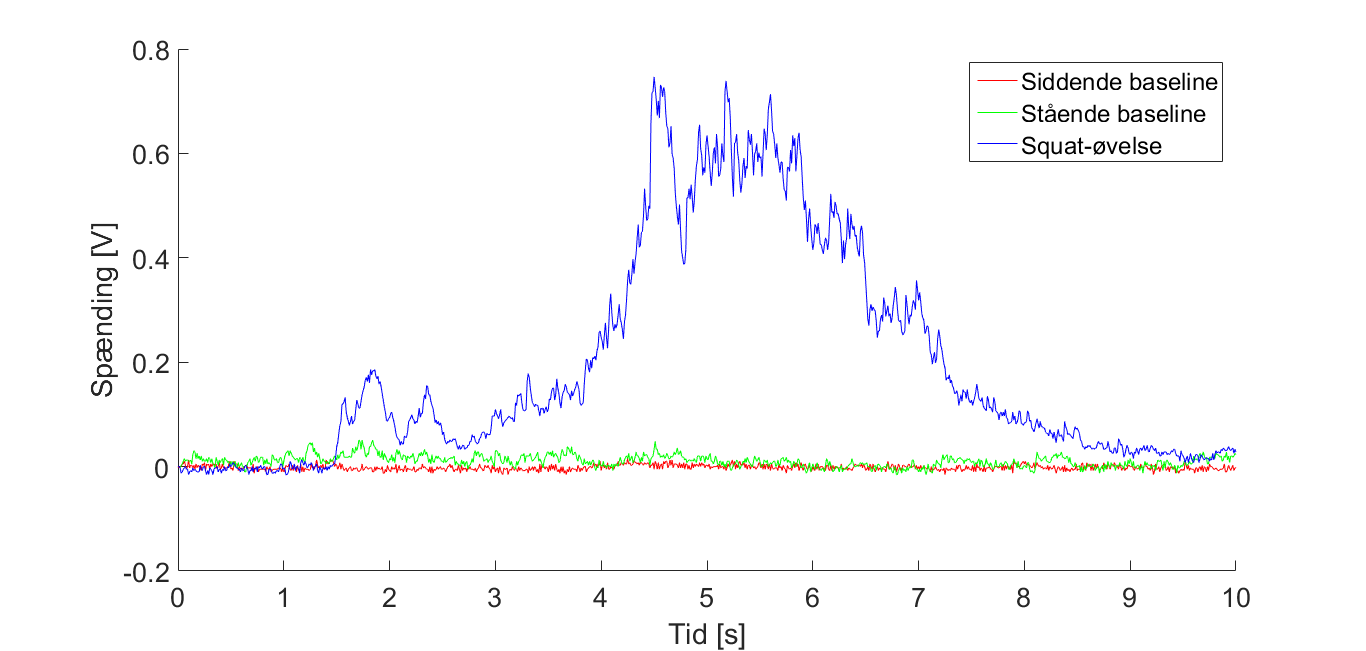
\includegraphics[width=0.85\textwidth]{figures/Pilotforsoeg/baselineogemg.png}
	\caption{EMG-målinger af baseline og 2. måling.}
	\label{fig:baselineogemg}
\end{figure}
Ud fra \autoref{fig:baselineogemg}, ses baseline samt 2. måling for forsøgsperson 1. Hertil ses et negativt offset for begge målinger mellem $0,5-0,6~V$. Ved 2. måling ses en stigning ved $1,5~s$, hvilket relateres til forsøgspersonens nedadgående bevægelse til maks $90^{\circ}$ flektion af knæet under squat-øvelsen. Yderligere ses et fald i amplitude ved ca. $6~s$, der relateres til en opdagående bevægelse til øvelsens udgangsposition. 


\begin{figure}[H]
	\centering
	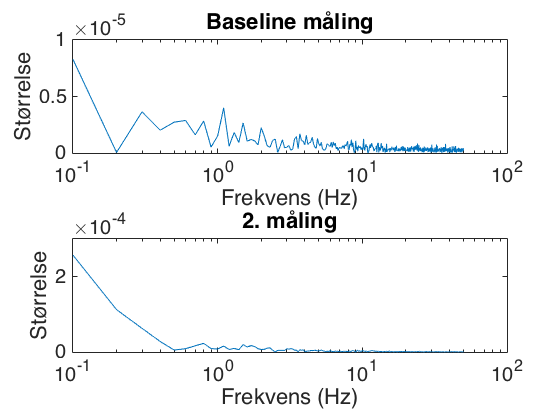
\includegraphics[width=0.85\textwidth]{figures/Pilotforsoeg/emgfft.png}
	\caption{Frekvensanalyse med semilogaritmisk skala på X-aksen af EMG-måling for baseline og 2. måling. Bemærk at der ikke er samme skalaer op af Y-aksen for de to grafer. Der ses derfor mere støj på 2. måling end baseline målingen.}
	\label{fig:emgfft}
\end{figure}

Der er foretaget en frekvensanalyse af baseline måling for at identificere støjsignaler. Dette ses af \autoref{fig:emgfft}, hvor der yderligere fremgår en frekvensanalyse af 2. måling for identificering af frekvensområdet for bevægelsen. For begge grafer er der foretaget en semilogaritmisk skala på X-aksen, hvilket resulterer i forskellige skalaer op af Y-aksen. Det ses ud fra målingerne et højere støjniveau på 2. måling end baseline målingen, dette støjniveau er dog relativt lav. 
Der observeres en DC-komponent ved $0~Hz$, hvilket svarer til det offset der er på signalet. 
Det fremgår ikke af figuren, hvorvidt der er $50~Hz$ støj på signalet, da der samples med $100~Hz$, hertil er Nyquist-frekvensen $50~Hz$. Herudover viser frekvensanalysen ikke amplituden af $50~Hz$ støj, dog antages den for at være tilstede, da dette er en kendt støjfaktor. 
Af frekvensanalysen for 2. måling identificeres frekvensområdet som værende relativt lavfrekvent $0.4-10~Hz$, hvorefter støjsignalerne dæmpes gradvist. Dette kan relateres til, at EMG-forstærkeren har en knækfrekvens på $1,94~Hz$, hvortil udregningen ses i \autoref{sec:sensorer}. 


\subsubsection{Resultater for accelerometer målinger} \label{sec:acc_fft}

\begin{figure}[H]
	\centering
	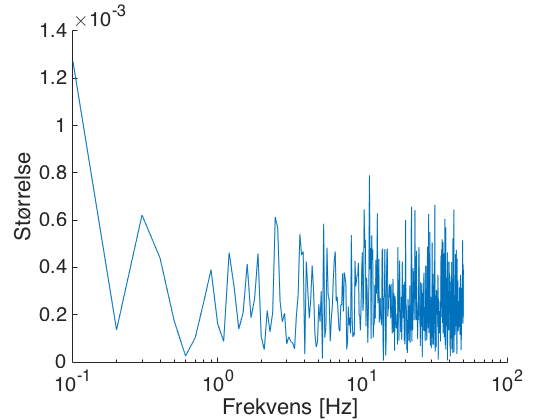
\includegraphics[width=0.85\textwidth]{figures/Pilotforsoeg/accfft.png}
	\caption{Frekvensanalyse af baseline måling for accelerometeret, hvor X-aksen er en semilogaritmisk skala}
	\label{fig:accfftx}
\end{figure}
Af \autoref{fig:accfftx} ses frekvensanalysen for accelerometeret i X-aksen. Ud fra dette ses yderligere støjsignaler end DC-komponent, der er dæmpet ved $0,1~Hz$. Grundet sampligsfrekvensen er der ingen $50~Hz$ støj, hvor årsagen er beskrevet under frekvensanalysen for EMG-målingen. 

Spændingerne fra accelrometeret repræsenterer vinklerne for femur og tibia i Y-aksen. Denne spændingsværdi ønskes omregnet til grader, for således at undersøge vinklen af knæet. Til at omregne spændingen fra begge acceleromtre til grader anvendes målingerne anvendt i \autoref{sec:resul_linear}. Disse resultater er anvendt i funktioner, hvor lineær interpolation benyttes. EMG-spændingerne for 2. måling er hertil anvendt i funktionerne, således graderne for EMG-målingen findes.
Resultaterne fra omregningen visualiseres af \autoref{fig:accvinkel}. 

\begin{figure}[H]
	\centering
	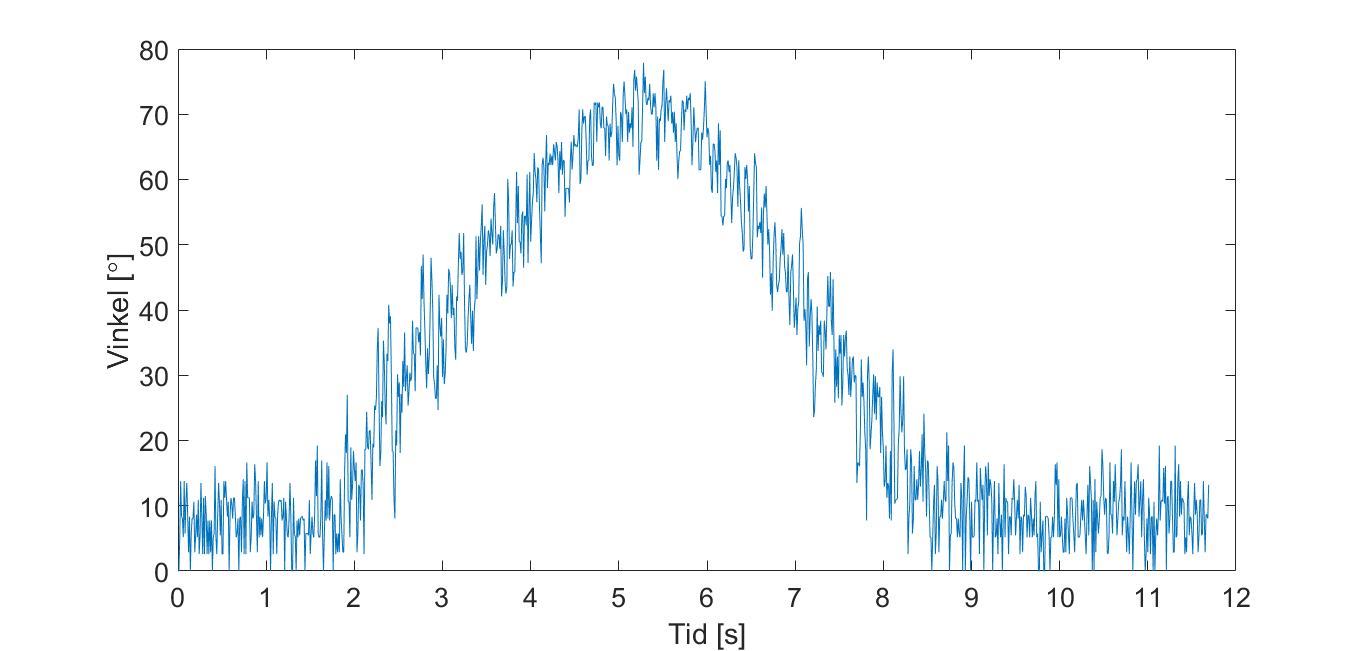
\includegraphics[width=0.8\textwidth]{figures/Pilotforsoeg/accvinkel}
	\caption{Vinkler fra accelerometrene under 2. måling}
	\label{fig:accvinkel}
\end{figure}
Det fremgår af \autoref{fig:accvinkel}, at forsøgspersonen udfører en fleksion af knæet under 2. måling når ned til en grad på ca. $78^{\circ}$. 

For at kunne se relationen mellem udslag i EMG samt for accelerometrene, plottes begge disse målinger på samme graf. Dette ses af \autoref{fig:emgogacc}. 
\begin{figure}[H]
	\centering
	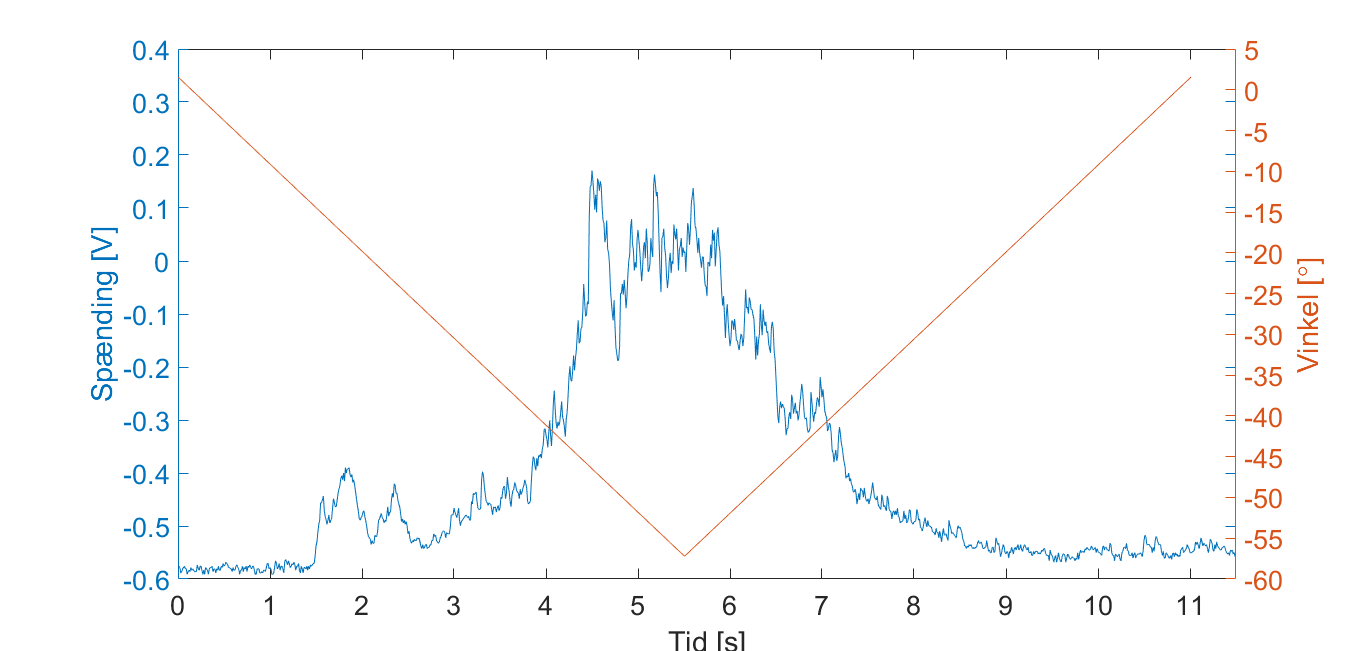
\includegraphics[width=0.8\textwidth]{figures/Pilotforsoeg/emg_vinkler_tid}
	\caption{EMG signal og vinkler fra acceleromtre under 2. måling}
	\label{fig:emgogacc}
\end{figure}


For at se sammenhængen mellem muskelaktivitet og de forskellige vinkler, plottes EMG signalerne som funktion af vinklerne. Det fremgår af \autoref{fig:emgogvinkel}, at der er en sammenhæng mellem vinklerne og mængden af muskelaktivitet. Ved fleksion bliver vinkelen større og muskelaktiviteten stiger dermed. Ved ekstension, hvor vinkelen bliver mindre, falder muskelaktiviten.





\begin{figure}[H]
	\centering
	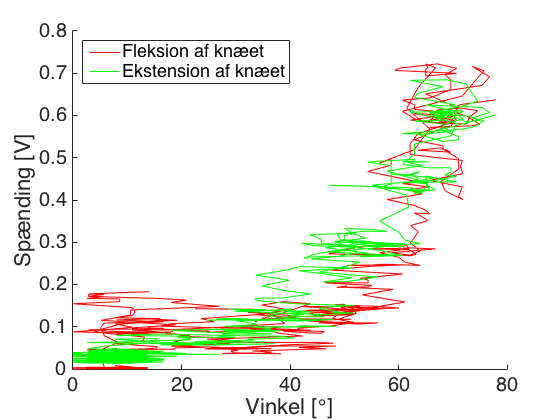
\includegraphics[width=0.8\textwidth]{figures/Pilotforsoeg/emg_vinkler}
	\caption{EMG målingen vist i forhold til vinkler}
	\label{fig:emgogvinkel}
\end{figure}



%\fxnote{OBS!!! Opsummeringen skal angiveligt omskrives!}
%\section{Opsummering af pilotforsøg}
%Af resultaterne fra databehandlingen ses det, hvilke parametre, der er nødvendige for optimeret drift af det endelige system. Ud fra frekvensanalysen af EMG-signalerne, ses ingen fremkomst af $50~Hz$ støj.\fxnote{Jeg ved ikke om vi kan antage dette, da frekvensanalysen reelt ikke viser 50 Hz.} Dette antages at skylde envalope kredsen i EMG-forstærkeren. Dette fungerer som et lavpasfilter, hvortil størrelsen af komponenterne i kredsen giver en knækfrekvens på ca. $2~Hz$. 
%
%Af frekvensanalysen fremkommer der dog en dc komponent, som følge af offsettet, der ses af EMG-målingerne. \fxnote{ønsker vi at fjerne det offset der fremgår i EMG-målingerne??} Dette giver anledning til, at implementere et højpasfilter, for således at dæmpe dc-komponenten. Dette skal dog være med visse forbehold, da frekvensanalysen yderligere viser, at signalerne er lavfrekvent. 
%
%Ved implementering af et højpasfilter, kan det ønskede signal dæmpes i for høj en grad, således signalet ikke vil være anvendeligt. 
% 
